
\part{结构强度}

\begin{tcolorbox}
    有一实心均温等厚轮盘,轮缘半径为 \qty{0.25}{\meter};其材料质量密度为 \qty{8000}{kg/m^3},泊松比
为 0.3,许用应力为 \qty{800}{MPa}。转子工作转速为 \qty{12000}{r/min},且轮缘受有 \qty{200}{MPa} 的外载
荷,通过计算回答下述问题:
    \begin{enumerate}
        \item 该实心轮盘能否安全工作?画出轮盘的应力分布曲线,即半径(Y 坐标)-径向应
        力曲线(X 坐标)以及半径(Y 坐标)-周向应力(X 坐标)曲线。
        \item 若因总体结构设计方案改变,需要在盘心处开一中心孔,问轮盘能否安全工作?
        若不能,如何改进设计?
        \item 若该实心轮盘盘心温度为 200 度、盘缘温度为 500 度,且温度沿着轮盘径向线性
        变化,试计算轮盘上的热应力分布。画出热应力分布曲线,即半径(Y 坐标)-径向应力
        曲线(X 坐标)以及半径(Y 坐标)-周向应力(X 坐标)曲线。弹性模量及线膨胀系数
        可取常数:$E=\qty{160}{GPa}, \alpha=\qty{18e{-6}}{\degreeCelsius^{-1}}$。
        \item 计算该实心轮盘总应力,并判断轮盘能否安全工作。画出总应力分布曲线,即半
        径(Y 坐标)-径向应力曲线(X 坐标)以及半径(Y 坐标)-周向应力(X 坐标)曲线。
    \end{enumerate}
\end{tcolorbox}

\section{第一题}

对于该问题,考虑使用位移法微分方程:
\begin{equation}
    \begin{aligned}
        \frac{\dif^2 u}{\dif r^2} + \left[ \frac{\dif}{\dif r} (\ln h )+ \frac{1}{r} \right] \frac{\dif u}{\dif r} + 
        \left[\frac{\nu}{r}\frac{\dif}{\dif r} (\ln h) - \frac{1}{r^2}\right] u & \\ 
        - (1 + \nu) \alpha \left[ t \frac{\dif}{\dif r} (\ln h) + \frac{\dif t}{\dif r}\right] +
        \rho \omega^2 \frac{1 - \nu^2}{E} r &= 0,
    \end{aligned}
\end{equation}
其中$r$为半径、$u$为位移、$h$为厚度、$t$为温度、$\omega$为角速度,$\nu, E, \rho, \alpha$分别为泊松比、杨氏模量、密度和线膨胀系数。
对等厚圆盘,有
\begin{equation}
    \frac{\dif h}{\dif r} = 0
\end{equation}
因此
\begin{equation}
    \begin{aligned}
        & \frac{\dif^2 u}{\dif r^2} + \frac{1}{r} \frac{\dif u}{\dif r} - \frac{u}{r^2} - (1 + \nu) \alpha \frac{\dif t}{\dif r} + \rho \omega^2 \frac{1 - \nu^2}{E} r = 0 \\
        \iff & \frac{\dif^2 u}{\dif r^2} + \frac{1}{r} \frac{\dif u}{\dif r} - \frac{u}{r^2} = (1 + \nu) \alpha \frac{\dif t}{\dif r} - \rho \omega^2 \frac{1 - \nu^2}{E} r \\
        \iff & \frac{\dif}{\dif r}\left( \frac{1}{r} \frac{\dif ru}{\dif r} \right) = (1 + \nu) \alpha \frac{\dif t}{\dif r} - \rho \omega^2 \frac{1 - \nu^2}{E} r.
    \end{aligned}
\end{equation}
积分,可得
\begin{equation}
    \frac{1}{r} \frac{\dif ru}{\dif r} = (1 + \nu) \alpha t- \frac{1 - \nu^2}{2E} \rho \omega^2 r^2 + C_1'.
\end{equation}
再次积分,得到
\begin{equation}
    ru = (1 + \nu) \alpha \int_{r_0}^r tr \dif r - \frac{1 - \nu^2}{8E} \rho \omega^2 r^4 + C_1 r^2 + C_2,
\end{equation}
其中$C_1', C_2$为积分常数,$C_1 = 2C_1'$.
根据本构方程(广义胡克定律),位移与应力之间具有以下关系:
\begin{equation}
    \begin{aligned}
        \epsilon_r = \frac{\dif u}{\dif r} &= \frac{\sigma_r - \nu \sigma_\theta}{E} + \alpha t, \\
        \epsilon_\theta = \frac{u}{r} &= \frac{\sigma_\theta - \nu \sigma_r}{E} + \alpha t.
    \end{aligned}
\end{equation}
代入并求解应力,可得
\begin{equation}
    \begin{aligned}
        \sigma_r &= K_1 - \frac{K_2}{r^2} -\frac{3+\nu}{8} \rho \omega^2 r^2 - \frac{\alpha E}{r^2} \int_{r_0}^r tr \dif r, \\
        \sigma_\theta & = K_1 + \frac{K_2}{r^2} -\frac{1+3\nu}{8} \rho \omega^2 r^2  - E \alpha t + \frac{\alpha E}{r^2} \int_{r_0}^r tr \dif r,
    \end{aligned}
    \label{equ:uniform-disk-stress}
\end{equation}
其中
\begin{equation}
    K_1 = \frac{C_1 E}{1-\nu}, K_2 = \frac{C_2 E}{1 + \nu},
\end{equation}
是两个根据边界条件求解的常数。
这个应力是由边界条件、离心载荷和热应力三个部分线性叠加组成的。

现在考虑题设实心圆盘的情况,有$r_0 = 0$,且边界条件为:
\begin{equation}
    \sigma_r (r_a) = \sigma_a,\; \sigma_r(0) = \sigma_\theta(0).
\end{equation}
从而解为
\begin{equation}
    \begin{aligned}
        K_1 & = \sigma_a + \frac{3+\nu}{8} \rho \omega^2 r_a^2 + \frac{\alpha E t_0}{2}, \\
        K_2 & = 0, \\
        \sigma_r & = \frac{3 + \nu}{8} \rho \omega^2 (r_a^2 - r^2) + \sigma_a, \\
        \sigma_\theta &= \frac{\rho \omega^2}{8} [(3+\nu) r_a^2 - (1+3\nu)r^2] + \sigma_a.
    \end{aligned}
\end{equation}
其中应力是由离心应力和边界条件两个部分线性叠加组成的。
现在带入数字即可,作图于图~\ref{fig:part-2-question-1}中。
可见最大应力小于许用应力,因此可安全工作。

\begin{figure}[!t]
    \centering
    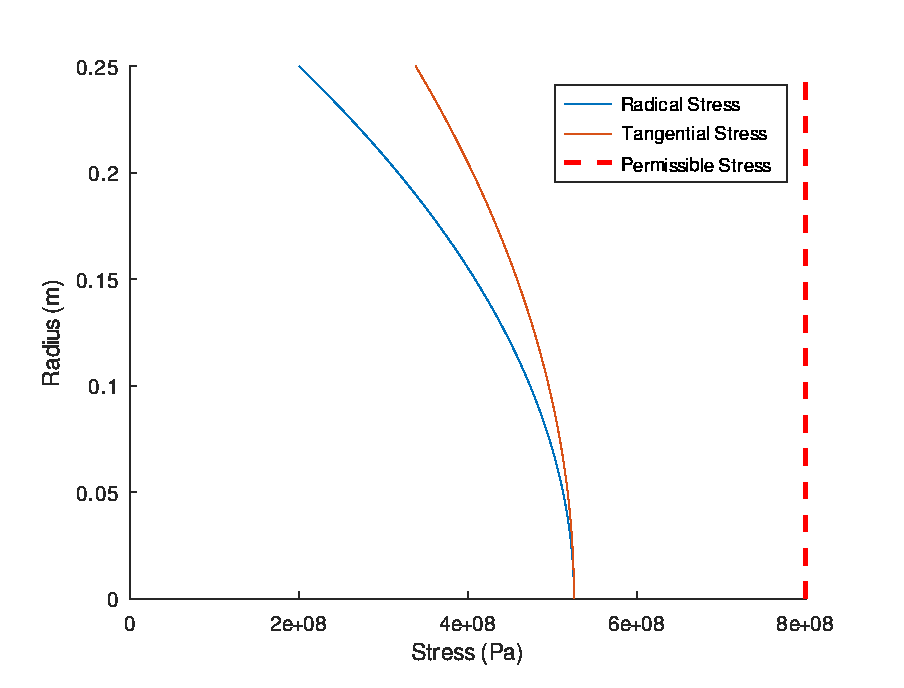
\includegraphics[width=0.8\linewidth]{part-2-question-1.eps}
    \caption{均温实心圆盘应力分布曲线。}
    \label{fig:part-2-question-1}
\end{figure}

\section{第二题}

对空心圆盘,边界条件变为
\begin{equation}
    \sigma_r (r_a) = \sigma_a,\; \sigma_r(r_0) = 0.
\end{equation}
其解为
\begin{equation}
    \begin{aligned}
        \sigma_r &= \frac{3 + \nu}{8} \rho \omega^2 \left( r_a^2 + r_0^2 - \frac{r_a^2 r_0^2}{r^2} - r^2\right) + \frac{r_a^2(r^2 - r_0^2)}{r^2(r_a^2 - r_0^2)}\sigma_a \\
        \sigma_\theta &= \frac{3+\nu}{8} \rho \omega^2 \left( r_a^2 + r_0^2 + \frac{r_a^2 r_0^2}{r^2} - \frac{1+3\nu}{3+\nu} r^2\right) + \frac{r_a^2(r^2 + r_0^2)}{r^2(r_a^2 - r_0^2)}\sigma_a.
    \end{aligned}
\end{equation}
该应力也是由离心应力和边界条件两个部分线性叠加组成的。
利用该解析解,可做出图~\ref{fig:part-2-question-2}。

\begin{figure}[!tb]
    \centering
    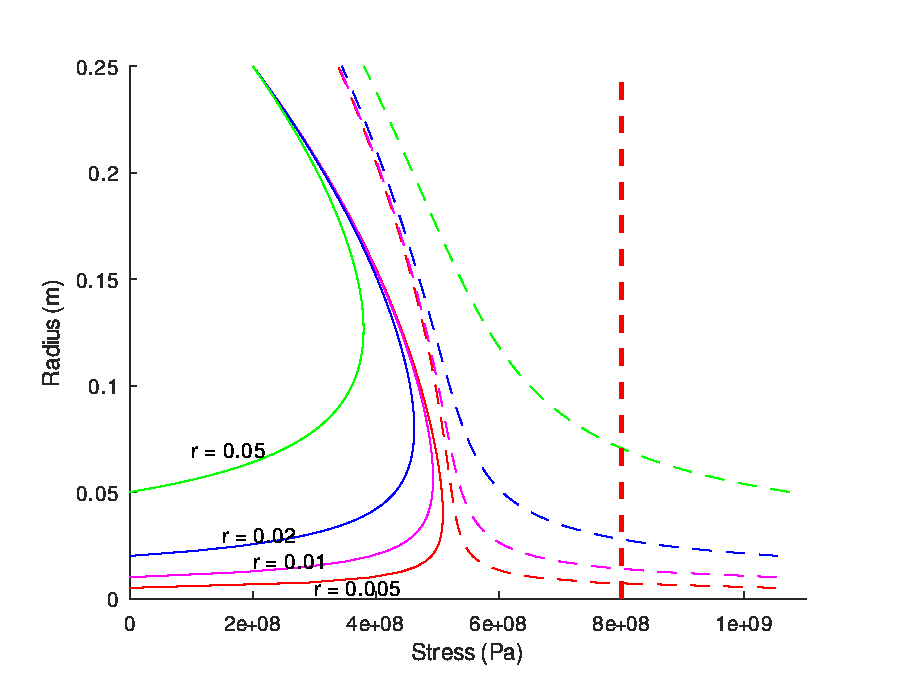
\includegraphics[width=\linewidth]{part-2-question-2.eps}
    \caption{均温空心圆盘应力分布曲线。实线:径向应力;虚线:切向应力。红色:内径\qty{0.005}{m};品红色:内径\qty{0.01}{m};蓝色:内径\qty{0.02}{m};绿色:内径\qty{0.05}{m}。}
    \label{fig:part-2-question-2}
\end{figure}

在圆盘内缘,径向应力为零,而切向应力为
\begin{equation}
    \sigma_\theta = 2 \left[ \frac{3 + \nu}{8} \rho \omega^2 \left( r_a^2 + \frac{1 - \nu}{3 + \nu} r_0^2\right) + \frac{r_a^2}{r_a^2 - r_0^2} \sigma_a \right].
\end{equation}
该应力关于内径单调递增,而当内径趋于零时该应力最小,为
\begin{equation}
    \lim_{r_0 \to 0} \sigma_\theta = \frac{3 + \nu}{4} \rho \omega^2 r_a^2 + 2 \sigma_a.
\end{equation}
根据题设带入数值,可得\(\sigma_{\theta, \min} = \qty{1051.39}{MPa}\),该数值大于许用应力,因此在任何内径下均不能安全使用该圆盘。

由于应力集中于边界处,可加厚该位置以提高边界处的强度,或选择更轻的材料以降低离心应力。也可选择强度更高的材料以提高许用应力。

\section{第三题}

式~\ref{equ:uniform-disk-stress}是由边界条件、离心载荷和热应力三个部分线性叠加组成的。
为求解热应力,我们考虑无载荷且静止的均匀圆盘,该式简化为
\begin{equation}
    \begin{aligned}
        \sigma_r &= K_1 - \frac{K_2}{r^2} - \frac{\alpha E}{r^2} \int_{r_0}^r tr \dif r, \\
        \sigma_\theta & = K_1 + \frac{K_2}{r^2} - E \alpha t + \frac{\alpha E}{r^2} \int_{r_0}^r tr \dif r.
    \end{aligned}
\end{equation}
对于实心无载荷的情况,有$r_0 = 0$且$\sigma_r(r_a) = 0, \sigma_\theta(0) = \sigma_r(0)$。
因此其热应力为
\begin{equation}
    \begin{aligned}
        K_1 &= \frac{\alpha E}{r_a^2} \int^{r_a}_0 tr \dif r, \\
        K_2 &= 0, \\
        \sigma_{r} &= \frac{\alpha E}{r_a^2} \int^{r_a}_0 tr \dif r - \frac{\alpha E}{r^2} \int_0^r tr \dif r, \\
        \sigma_\theta &= \frac{\alpha E}{r_a^2} \int^{r_a}_0 tr \dif r + \frac{\alpha E}{r^2} \int_0^r tr \dif r - E \alpha t.
    \end{aligned}
\end{equation}

根据题设,温度沿轮盘径向线性变化,因此设
\begin{equation}
    t(r) = kr + t_0.
\end{equation}
代入求解,得
\begin{equation}
    \begin{aligned}
        \sigma_{r} &= \frac{\alpha k E}{3} (r_a - r),\\
        \sigma_\theta &= \frac{\alpha k E}{3} (r_a - 2 r).
    \end{aligned}
\end{equation}
代入数值即可做出图~\ref{fig:part-2-question-3}。

\begin{figure}[!tb]
    \centering
    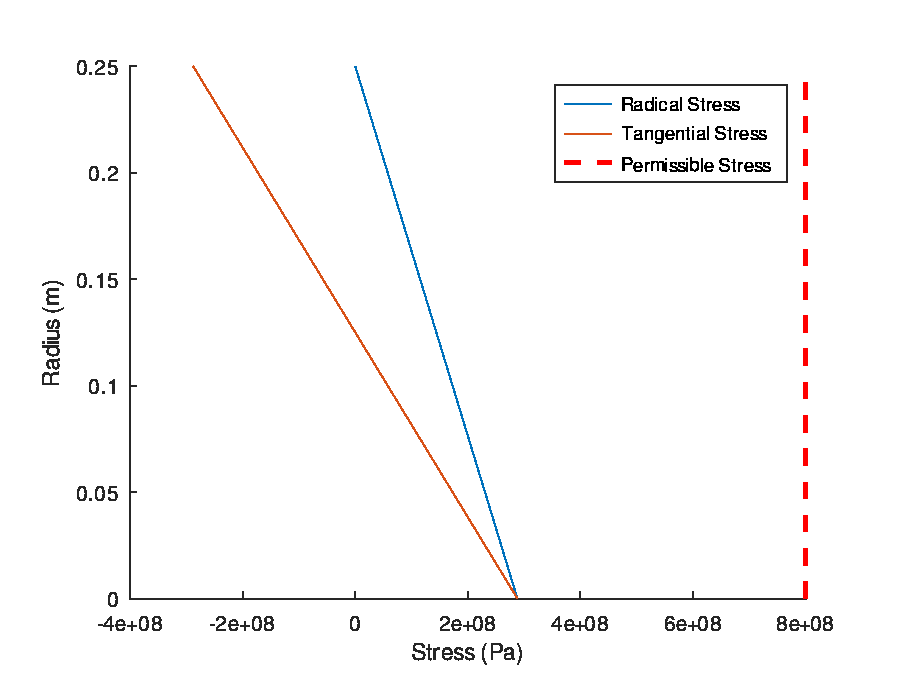
\includegraphics[width=0.8\linewidth]{part-2-question-3.eps}
    \caption{实心圆盘线性热载荷下的热应力。}
    \label{fig:part-2-question-3}
\end{figure}

\section{第四题}

利用叠加原理,将热应力与前文的结果相加,即可得到总应力,如图~\ref{fig:part-2-question-4}所视。
观察图示容易看出,圆盘在热载荷下的总应力超过了许用应力,因此不能安全工作。

\begin{figure}[!tb]
    \centering
    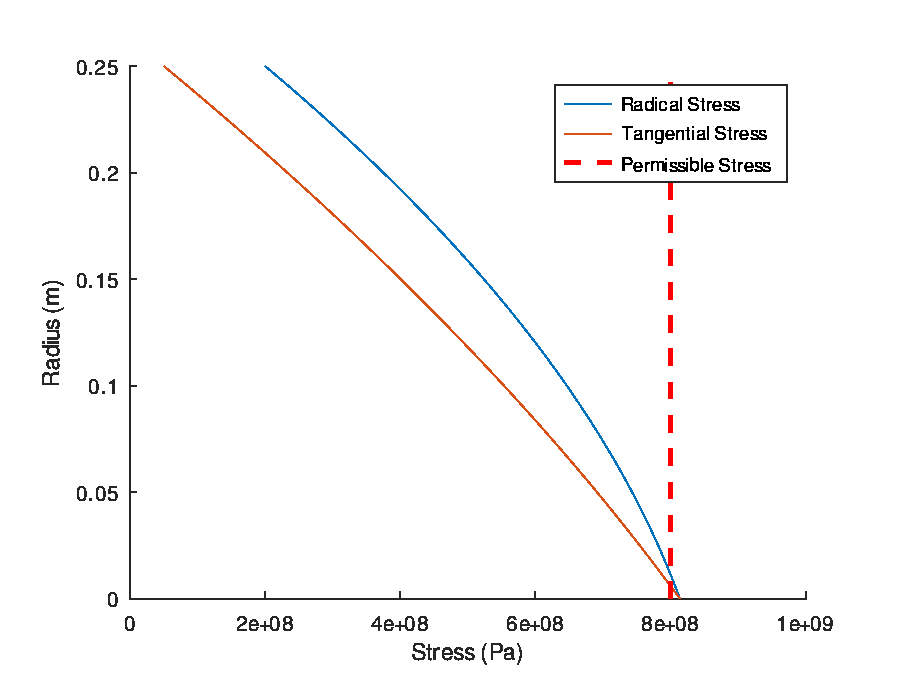
\includegraphics[width=0.8\linewidth]{part-2-question-4.eps}
    \caption{实心圆盘线性热载荷下的总应力。}
    \label{fig:part-2-question-4}
\end{figure}
